%
% main.tex -- Paper zum Thema komplexe Morlet Wavelets und CWT
%
% (c) 2019 Hochschule Rapperswil
%

\chapter{Komplexe Morlet Wavelets und CWT\label{chapter:complex}}
\lhead{Komplexe Wavelets und CWT}
\begin{refsection}
\chapterauthor{Roy Seitz}

% \section{Einleitung}
Die diskrete Wavelet-Transformation (DWT) mit reellen Wavelets ist besonders schnell zu berechnen.
Deshalb ist sie die bevorzugte Wahl bei allen Signalverarbeitungs-Anwendungen.
Beim Erstellen `schöner' Bilder trifft man jedoch auf folgende drei Probleme:

Erstens wäre es für Bilder vorteilhaft, die relevanten Frequenzpunkte vorgeben zu können.
So kann man direkt lineare oder logarithmische Skalen wählen. Die DFT ist an Zweierpotenzen gebunden.
Zweitens erfordern die gängigsten Methoden zum Erstellen von Bildern ein reguläres Raster, also in jede Zeile dieselbe Anzahl Pixel.
Möchte man Schwingungen finden, ist es zudem vorteilhaft, wenn das Bild proportional zur Amplitude ist, also Phasen-unabhängig.
Bei reellen Wavelets sind Amplitude und Phase jedoch nicht einfach zu trennen.

Die CWT aus Kapitel~\ref{chapter:cwt} ist die bevorzugte Wahl für analytische Berechnungen.
Als kontinuierliche Transformation ist sie jedoch sehr rechenintensiv und benötigt etwas Vorarbeit,
nämlich eine Diskretisierung der $a$- und $b$-Variablen.
Eine anschliessende direkte Berechnung der diskretisierten Integrale ist ineffizient.
Im ersten Abschnitt betrachten wir deshalb, wie man die CWT als Faltung interpretieren kann, welche sich effizient mittels FFT berechnen lässt.
Zur Illustration verwenden wir ein einfaches Beispielsignal und die CWT mittels Haar-Wavelet.

Die Wahl des Wavelets spielt eine zentrale Rolle und beeinflusst das erhaltene Bild wesentlich.
Ein wichtiger Punkt ist hierbei die Unschärfe-Relation zwischen Zeit und Frequenz.
Ein Signal kann nicht in beidem zugleich gut lokalisiert sein.
Im zweiten Abschnitt vergleichen wir deshalb die CWT mittels Haar- und Gabor-Wavelet anhand zweier Beispielsignale.

Im dritten Abschnitt wenden wir uns den komplexen Wavelets zu.
Via Hilbert-Transformation können wir basierend auf einem beliebigen Wavelet ein neues finden, bei welchem sich Phasen und Amplitude trennen lassen.

Durch die Berechnung der CWT mittels FFT entstehen Artefakte am Bildrand durch die zirkuläre Faltung.
Geschickte Erweiterung des Signals kann diesen Effekt vermeiden.
Dies beeinflusst jedoch massgeblich die Performance, da durch Erweitern des Signals der Rechenaufwand signifikant steigt.
Im letzten Abschnitt vergleichen wir deshalb den Rechenaufwand und die erzielten Bilder mit verschiedenen Padding-Optionen anhand eines Matlab-Skripts.
Zudem vergleichen wir die Performance dieses Skripts mit der Implementation von Matlab selbst.
Überraschenderweise ist es auf den getesteten Rechnern in jedem Fall schneller als die cwt-Funktion aus der Wavelet-Toolbox von Matlab.

%%%%%%%%%%%%%%%%%%%%%%%%%%%%%%%%%%%%%%%%%%%%%%%
\section{Effiziente Berechnung der CWT}
\rhead{Berechnung der CWT}
Als erstes möchten wir herausfinden, wie sich die CWT effizient berechnen lässt.
Als zweites werden wir zwei Beispielsignale definieren und die CWT mittels Haar-Wavelet betrachten.
Abschliessend rechnen wir die CWT noch mit dem Gabor-Wavelet und vergleichen die beiden Bilder.

\subsection{CWT als Faltung}
Betrachten wir zuerst die folgende Gleichung
\begin{equation}
\Wave f (a,b)
=
\langle f,\psi_{a,b}\rangle
=
\frac{1}{\sqrt{|a|}}\int_{-\infty}^\infty f(t)\,
	\overline{\psi}\biggl(\frac{t-b}{a}\biggr)\,dt,\label{complex:CWT}
\end{equation}
durch welche in Definition~\ref{cwt:definition} die kontinuierliche Wavelet-Transformation eingeführt wurde.
Dieses Integral entspricht der Faltung zwischen $f(t)$ und 
\begin{equation} 
    g(t) 
    = \frac{1}{\sqrt{|a|}} \overline\psi\biggl(\frac{-t}{a}\biggr).
\end{equation}
Der Standard-Trick zur effizienten Berechnung einer Faltung ist die Multiplikation im Frequenzbereich.
\begin{equation} 
\mathcal{W}f (a,b) = (f*g)(t) = \mathcal{F}^{-1}\biggl\lbrace\hat f(\omega) \hat g (\omega) \biggr\rbrace.
\end{equation}
Dafür benötigen wir die Fouriertransformierte $\hat g (\omega)$:
\begin{align*}
	\hat g (\omega) = 
    \Four\,\biggl\lbrace \frac{1}{\sqrt{|a|}} \overline\psi \biggl(\frac{-t}{a}\biggr) \biggr\rbrace 
	&= \frac{1}{\sqrt{|a|}} \int_{-\infty}^{\infty}\overline\psi\biggl(\frac{-t}{a}\biggr) \, e^{-i\omega t}\,dt\\
	&= \frac{1}{\sqrt{|a|}} \overline{\int_{-\infty}^{\infty}\psi \biggl(\frac{-t}{a}\biggr) \, e^{i\omega t}\,dt}  
    & \biggl(\text{Substitution } t' = \frac{-t}{a}\biggr)\\
	&= \frac{1}{\sqrt{|a|}} \overline{\int_{-\infty}^{\infty}\psi(t') \, e^{-ia\omega t'} |a|\,dt'}\\
	&= \sqrt{|a|} \, \overline{\hat{\psi}}(a\omega).
\end{align*}
Gleichung~\eqref{complex:CWT} lässt sich somit schreiben als
\begin{equation}
\Wave f(a,b)
= \mathcal{F}^{-1}\bigl\lbrace\hat{f}(\omega) \sqrt{|a|}\, \overline{\hat{\psi}}(a\omega)\bigr\rbrace. \label{complex:fcwt}
\end{equation}

Mittels Fourier-Transformation lässt sich die Wavelet-Transformation folglich besonders elegant berechnen.
Kontinuierliche Funktionen sind für numerische Systeme jedoch ungeeignet.
Die CWT muss in $a$ und $b$ diskretisiert werden.
Die Diskretisierung von $b$ entspricht vorteilhaft gerade derjenigen des Signals selbst.
Dann lässt sich die Fourier-Transformation mittels FFT effizient berechnen und Gleichung~\eqref{complex:fcwt} wird zu
\begin{equation}
	\mathcal{W}f(a,b) = \text{IFFT}\bigl(\text{FFT}(f) \, \overline{\hat{\psi}}(a\omega)\bigr). \label{complex:ffcwt}
\end{equation}

Der Faktor $\sqrt{|a|}$ wurde hierbei weggelassen.
Hierdurch werden die hohen Frequenzen stärker gewichtet und $|\!\Wave f(a,b)|$ ist gerade proportional zur Amplitude der analysierten Signalkomponente.
Zudem erzielen wir im Diskreten nicht exakt die Faltung, sondern die zirkuläre Version davon. 
Mehr dazu im Abschnitt~\ref{complex:circ-conv-padding}.

Gleichung~\eqref{complex:ffcwt} muss für jedes $a$ einzeln gelöst werden.
Sie wird besonders interessant, wenn das Wavelet im Frequenzbereich eine geschlossene, analytische Form besitzt.
Dann benötigt man nur eine FFT für das Signal, so wie für jedes $a$ eine inverse FFT und eine punktweise Multiplikation zwischen Signal und Wavelet.

%\clearpage
\subsection{Das Haar-Wavelet}
\rhead{Haar-Wavelet}
\begin{figure}
	\centering
	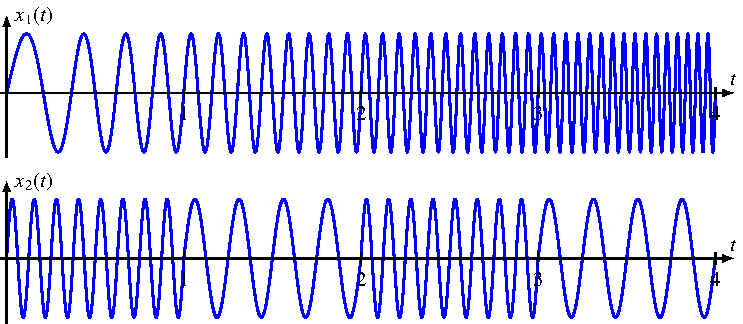
\includegraphics{papers/complex/images/signals.pdf}
	\caption{Die beiden Beispielsignale $x_1(t)$ und $x_2(t)$}
\end{figure}
Rechnen wir das erste Beispiel.
Hierfür benötigen wir zwei Dinge: Signal und Wavelet.
Als Signale nehmen wir zwei Sinus-Schwingungen, eine mit linear ansteigender und eine mit stückweise konstanter Frequenz.
\begin{align}
    x_1(t) &= \sin\left( \int_{0}^{t} 2\pi f_1(\tau)\,d\tau\right) & f_1(t) &= 2 + 6/4 \cdot t \\
    x_2(t) &= \sin\left( \int_{0}^{t} 2\pi f_2(\tau)\,d\tau\right) & f_2(t) &= \left\lbrace \begin{matrix}
    4, & &t& < 1\\
    8, & 1.0 \le &t& < 2.0\\
    4, & 2.0 \le &t& < 3.0\\
    8, & 3.0 \le &t&\\
    \end{matrix}\right.
\end{align}
Das Haar-Wavelet sei in diesem Abschnitt zentriert um $t=0$.
Die daraus resultierende Symmetrie wird sich in der Berechnung der Fourier-Transformation als hilfreich erweisen.

\begin{definition}
	\label{complex:def-haar-wavelet}
	Das Haar-Wavelet besitzt folgende Gestalt:
	\[
	\psi_{\text{Haar}}(t) = \left\lbrace\begin{matrix*}[r]
	1 & -\frac{1}{2} \le t < 0  \\
	-1 & 0 \le t < \frac{1}{2} \\
	0 & \text{sonst}.
	\end{matrix*} \right.\label{complex:def-haar}
	\]
\end{definition}
Die Fourier-Transformierte von $\psi_{\text{Haar}}$ berechnet sich wie folgt:
\begin{align}
	\Four \psi_\text{Haar}  
	&= \frac{1}{\sqrt{2\pi}}\int_{-\infty}^{\infty} \psi_\text{Haar} e^{-i\omega t} \,dt\nonumber\\
	&= \frac{1}{\sqrt{2\pi}}\Biggl( \int_{-1/2}^{0} e^{-i\omega t} \,dt - \int_{0}^{1/2} e^{-i\omega t}\,dt \Biggr) \nonumber\\
	&= \frac{i}{\sqrt{2\pi}\omega}\bigl( \bigl[ e^{-i\omega t}\bigr]_{-1/2}^0  - \bigl[ e^{-i\omega t}\bigr]_{0}^{1/2} \bigr)\nonumber\\
	&= \frac{i}{\sqrt{2\pi}} \frac{1-\cos(\omega/2)}{\omega/2}\label{complex:f-psi-haar}
\end{align}
Das Haar-Wavelet ist also nicht nur im Zeit-, sondern auch im Frequenzbereich besonders einfach.
Insbesondere lässt sich die mit $a$ skalierte Version des Wavelets durch Satz~\ref{four-int:trans-dial} direkt im Frequenzbereich berechnen.
Abbildung~\ref{complex:haar} zeigt das Haar-Wavelet im Zeit- und Frequenzbereich.
Auffallend ist, dass das im Zeitbereich besonders gut lokalisierte Haar-Wavelet in der Frequenz sehr schlecht lokalisiert ist.
\begin{figure}
	\centering
	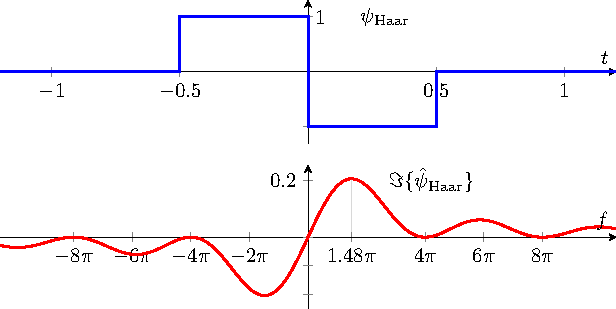
\includegraphics{papers/complex/images/haar.pdf}
	\caption{Das Haar-Wavelet}
	\label{complex:haar}
\end{figure}

\begin{figure}
	\centering
	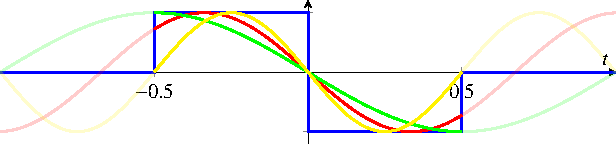
\includegraphics{papers/complex/images/haar_dom.pdf}
	
	\caption{Blau: $\psi_\text{Haar}$, Rot: $\sin ({\color{red}\omega_\psi}\cdot t)$, Gelb: $\sin ({\color{yellow}1.0}\cdot 2\pi t)$, Grün: $\sin ({\color{green}0.5}\cdot 2\pi t)$}
	\label{complex:dom-freq}
\end{figure}
An dieser Stelle definieren wir noch die \emph{dominante Frequenz} eines Wavelets.
\index{dominante Frequenz}%
\begin{definition}
	Die Fourier-Transformierte eines Wavelets erreicht den maximalen Betrag bei der \emph{dominanten Frequenz $\omega_\psi$}.
	\begin{equation}
		\omega_\psi \coloneqq \underset{\omega}{\text{\emph{argmax}}} \, |\hat\psi(\omega)|
	\end{equation}
	
\end{definition}

Die dominante Frequenz erlaubt, die $a$-Achse der Wavelet-Transformation als Frequenz-Achse zu interpretieren.
Für die Momentanfrequenz gilt
\[
	\omega(b) \approx \frac{\omega_\psi}{a_\text{max}(b)},
	\qquad 
	a_\text{max}(b)
	= 
	\underset{a}{\text{argmax}} \, |\!\Wave f(a,b)|.
\]
Diese Interpretation ist natürlich nur zulässig, wenn das Signal zum betrachteten Zeitpunkt nur eine dominante Frequenz-Komponente beinhaltet.
Bei unseren Beispielsignalen ist dies der Fall.
Abbildung~\ref{complex:dom-freq} illustriert die Bedeutung von $\omega_\psi$ für das Haar-Wavelet.
Es ist die Frequenz, bei welcher das Skalarprodukt mit dem Wavelet maximal wird.

Somit haben wir für unser Beispiel alles zusammen.
Nach einer Diskretisierung der Variablen überlassen wir die Arbeit dem Computer.
Dies liefert die Bilder aus Abbildung~\ref{complex:haar-ex}.

\begin{figure}
	\centering
	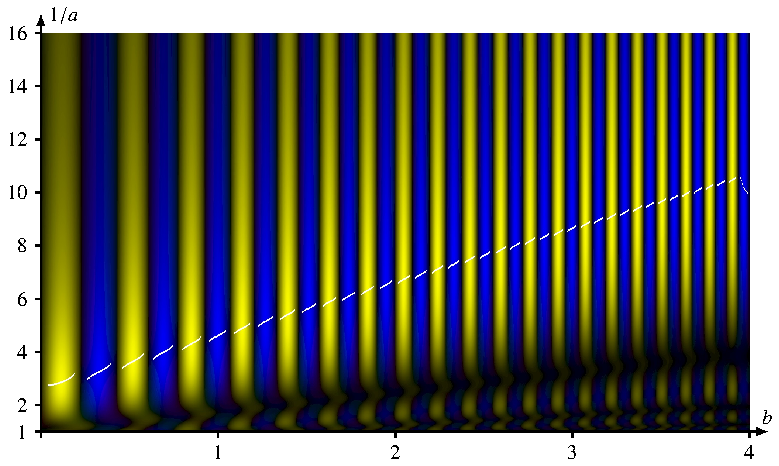
\includegraphics{papers/complex/images/chirp_haar.pdf}
	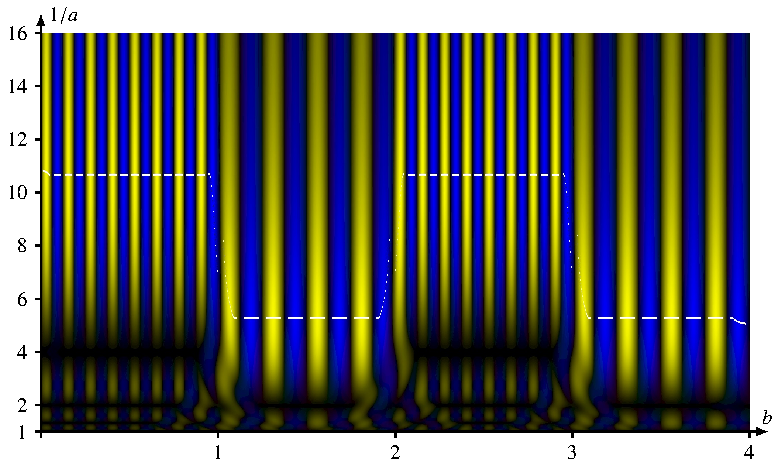
\includegraphics{papers/complex/images/square_haar.pdf}
	\caption{Wavelet-Transformationen der beiden Beispielsignale mit dem Haar-Wavelet. 
		Die Lokalisierung in der Zeit ist sehr gut, aber die momentane Frequenz ist kaum ersichtlich. 
		Zudem resultiert das periodische Signal in einer periodischen Helligkeit. 
		(Zur Erinnerung: bei reellen Werten entspricht die Farbe dem Vorzeichen, Blau: $+$, Gelb $-$)
	}
	\label{complex:haar-ex}
\end{figure}

Wie erwartet ist die Lokalisierung in der Frequenz ziemlich schlecht.
Das Haar-Wavelet gibt den Zeitpunkt einer Änderung der Frequenz zwar sehr genau wieder, die Frequenz selbst ist jedoch kaum ablesbar.
Als Orientierungshilfe sind $a_\text{max} (b) = \max_a{|\!\Wave x_n(a,b)|}$ weiss hervorgehoben.
Sie weichen um $\omega_\psi$ von der Signal-Frequenz ab, welche als Schwingung in der Amplitude gut erkennbar ist.
Dieses An- und Abschwellen des Betrags der Skalarprodukte verhindert es, $a_\text{max}(b)$ einfach zu folgen.
Dies werden wir im Abschnitt~\ref{complex:separate} durch komplexe Wavelets beheben.
Zuerst kümmern wir uns aber um die Lokalisierung in der Frequenz.


\section{Das Morlet-Wavelet}
\rhead{Morlet Wavelet}
Auch die reellen Fourierreihen haben das Problem, dass man Amplitude und Phase nicht separat betrachten kann, wenn man nur die Cosinus-Terme verwendet.
Dies liegt daran, dass Amplitude und Phase beim Cosinus gekoppelt sind,
\[
x = A\cos(\alpha) \quad\leftrightarrow\quad \alpha = \cos^{-1}\left(\frac{x}{A}\right).
\]
Erst durch die komplexe Schwingung 
\begin{align*}
	z(t) = Ce^{i\omega t} &= |C|e^{i\left(\omega t + \arg C\right)}
%	 &= |C|\left[\cos\left(\omega t + \arg C\right) + i \sin\left(\omega t + \arg C\right)\right]
\end{align*}
erhält man eine Basisfunktion, die mit
\[
	|z(t)| = |C| \quad \text{und}\quad
	\arg z = \arg \omega t + \arg C
\]
eine separate Betrachtung von Amplitude und Winkel erlaubt.
Diese Eigneschaft überträgt sich von den Basisfunktionen auf die Fouriertransformation.
Aufgrund der eulerschen Formel
\begin{equation}
	\cos(x) = \frac{e^{ix} + e^{-ix}}{2}\label{complex:euler}
\end{equation}
kann der Cosinus aus zwei komplexen Exponentialfunktionen mit inverser Frequenz dargestellt werden.
Besitzt ein Wavelet also negative Frequenz-Anteile, dann geht bei diesen Frequenzen die Eigenschaft der Separierbarkeit von Amplitude und Phase verloren.

\begin{figure}
	\centering
	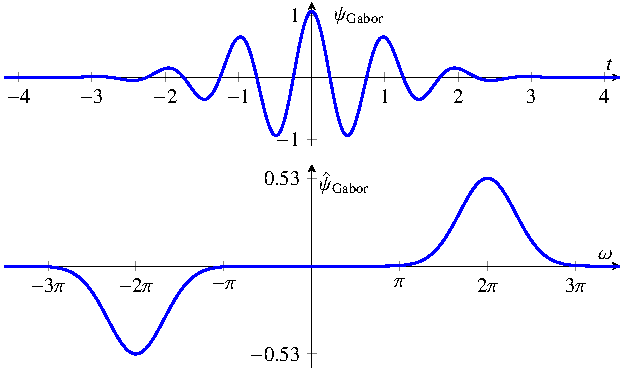
\includegraphics{papers/complex/images/gabor.pdf}
	\caption{Das Gabor-Wavelet für $\sigma = 2\pi$ \label{complex:gabor}}
\end{figure}

Ein geeignetes Wavelet benötigt folglich eine Fouriertransformierte, die bei negativen Frequenzen verschwindet.
Betrachten wir nun das Gabor-Wavelet
\[
	\psi = c_\sigma e^{-\frac{t^2}{2}}\left(\cos\left(\sigma t\right) - \kappa_\sigma\right),
\]
welches auch in Abbildung~\ref{complex:gabor} ersichtlich ist.
$c_\sigma$ und $\kappa_\sigma$ sind hierbei positive, reelle Konstanten, welche die Norm und die Zulässigkeitsbedingung~\eqref{cwt:zulaessig} korrigieren.
$\kappa_\sigma$ ist typischerweise sehr klein und wird oftmals einfach weggelassen.
Dieses Wavelet besitzt die dominante Frequenz $\sigma$ und ist durch die Gaus-Funktion in der Zeit lokalisiert.
Das Gabor-Wavelet eignet sich deshalb besonders gut, um einzelne Frequenzen in einem Signal zu finden.

Durch die Cosinus-Funktion besitzt das Gabor-Wavelet jedoch negative Frequenzen, wodurch eine isolierte Betrachtung von Amplitude und Phase unmöglich wird.
Dies möchten wir im Folgenden korrigieren.
Hierzu wechseln wir in den Fourierbereich.
Wir nutzen aus, dass die Fouriertransformierte einer Gaus-Kurve wieder eine Gauskurve ist,
\[
	\mathcal{F}\left\lbrace e^{-\alpha x^2} \right\rbrace 
	= \frac{1}{\sqrt{2\alpha}}e^{- \frac{\omega^2}{4\alpha}},
\]
und dass die Multiplikation im Zeitbereich zur Faltung im Frequenzbereich wird.
Zudem verwenden wir die Eulerformel~\eqref{complex:euler}.
Die Fouriertransformeirte des Gabor-Wavelet wird hierdurch zu
\[
 \hat{\psi} = 
 c_\sigma e^{- \frac{\omega^2}{2}} * \left(
  \frac{1}{2}\delta(\omega - \sigma) +
  \frac{1}{2}\delta(\omega + \sigma) + 
  \kappa_\sigma\delta(\omega)
  \right).
\]
Hierbei bezeichnet $\delta(\omega)$ die Dirac-Distribution.
Hieraus lässt sich der negative Anteil des Cosinus leicht entfernen.
Zudem verdoppeln wir den Anteil der positiven Frequenzen (der Grund hierfür erschliesst sich im nächsten Kapitel).
Wir erhalten
\[
	\hat{\psi}^\ast = 
	c_\sigma e^{- \frac{\omega^2}{2}} * \left(
	\delta(\omega - \sigma) +
	\kappa_\sigma\delta(\omega)
	\right),
\]
und durch Rücktransformation in den Zeitbereich
\[
	\psi^\ast = 
	c_\sigma e^{- \frac{t^2}{2}} \cdot \left(
	e^{i\sigma t} +
	\kappa_\sigma
	\right).
\]
Dies ist ein alter Bekannter, das Morlet-Wavelet aus Gleichung~\eqref{cwt:morlet}.
Abbildung~\ref{complex:morlet} zeigt den Real- und Imaginärteil, so wie die Envelope des Morlet-Wavelets.
Die Unabhängigkeit der Amplitude und der Phase 
Die Envelope entspricht hierbei gerade dem Absolutwert.
Das Morlet-Wavelet eignet sich also besonder gut, um bestimmte Frequenzen in einem Signal zu lokalisieren.
Im nächsten Kapitel werden wir sehen, dass man aus jedem, reellen Wavelet eines konstruieren kann, welches eine separate Betrachtung von Amplitude und Phase ermöglicht.

\begin{figure}
	\centering
	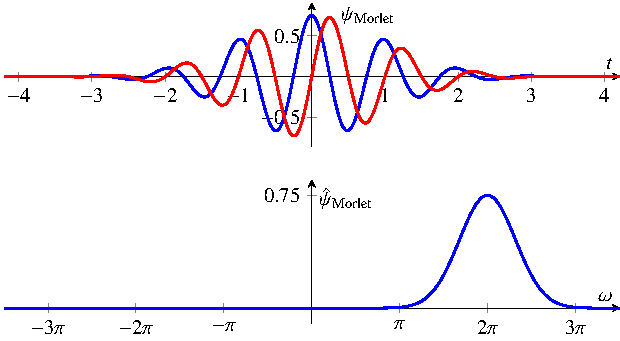
\includegraphics{papers/complex/images/morlet.pdf}
	\caption{Real- (blau) und Imaginärteil (rot) des Morlet-Wavelet für $\sigma = 2\pi$ \label{complex:morlet}}
\end{figure}

\section{Analytische Wavelets und Hilbert-Transformation}
\section{Analytische Wavelets}
Im vorherigen Abschnitt haben wir negative Frequenzen als Problem identifiziert.
Am Beispiel des Gabor-Wavelets suchten wir eine Lösung und fanden so das Morlet-Wavelet.
Dazu mussten alle negativen Frequenzen aus dem Spektrum des Wavelets entfernt werden.
Wie lässt sich dieses Verfahren veralgemeinern? 

Die Signaltheorie kennt genau dieses Verfahren in der Einseitenband-Modulation.
Wir entlehnen uns von dort den Begriff des \emph{analytischen Signals}\footnote{
	Der Begriff `analytisch' ist in diesem Kapitel immer im Sinne der Signaltheorie zu verstehen, also $\forall \omega < 0 \colon \hat f (\omega) = 0 $.
	Er ist nicht zu verwechseln mit der Eigenschaft analytischer Funktionen in der Analysis.
}
und defineiren analog dazu \emph{analytische Wavelets}.

\subsection{Analytische Signale und die Hilbert-Transformation}
\rhead{Hilbert-Transformation}
Bevor wir den Begriff des analytischen Signals einführen können, benötigen wir die Hilbert-Transformation
\[
\Hilb f(t) =
\frac{1}{\pi} \CH\int_{-\infty}^{\infty}\frac{f(x)}{t-x} \mathrm{d}x.
\]
Hierbei bezeichnet $\CH\int_{-\infty}^{\infty} \dots \mathrm{d}x$ den cauchysche Hauptwert des divergenten Integrals.
Diese Integral-Transformation wird uns erlauben, zu einem reellen Signal einen Imaginärteil zu finden, so dass gerade alle negativen Frequenzen im verscheinden.
Damit sind wir bereit für die Definition des analytischen Signals.

\begin{satz}
	\label{complex:analytic-signal}
	Sei $f(t) \in \mathbb{R}$ ein reelles Signal, dann heisst
	\begin{align*}
		f^\ast(t) 
		&= (1 + i\Hilb\,)f(t)
	\end{align*}
	das $f(t)$ zugeordnete \emph{analytische Signal}.
	Die Fourier-Transformierte eines analytischen Signals verschwindet für alle negativen Frequenzen.
	\[
		\forall \omega < 0 \colon \hat{f}^\ast(\omega) = 0
	\]
\end{satz}

\begin{proof}[Beweis]
	
	Die Hilbert-Transformation besitzt die Form eines Faltungs-Integrals.
	Im Frequenzbereich wird daraus eine Multiplikation.
	Es gilt mit der Signumsfunktion $\sgn(\omega)$ und der Identität
	\begin{align*}
		\Four \frac{1}{\pi t}  &= -i\sgn(\omega), \\
		\Hilb f(t) &= \frac{1}{\pi t} * f(t)\\
		\Four\Hilb f(t) &= -i\sgn(\omega) \hat{f}(\omega).
	\end{align*}
	Für die Fourier-Transformierte $\hat f^\ast(\omega)$ gilt folglich 
	\begin{align*}
		\hat{f}^\ast(\omega) 
		&= \hat{f}(\omega) - i^2\sgn(\omega)\hat{f}(\omega)\\
		&= (1 +\sgn(\omega))\hat{f}(\omega)\qedhere
	\end{align*}
\end{proof}

\begin{lemma}\label{complex:re-f-ast}
	Die Realteile von $f(t)$ und $f^\ast(t)$ sind identisch.
\end{lemma}

\begin{proof}
	Die Hilbert-Transformation ist eine reelle Integraltransformation
	\[\Hilb\,\colon\mathbb{R}\to\mathbb{R}.\]
	Folglich gilt nach Definition
	\[\Re f^\ast(t) = f(t) \quad \text{und}\quad \Im f^\ast(t) = \Hilb f(t)\qedhere\]
\end{proof}
Lemma~\ref{complex:re-f-ast} hält fest, dass wir uns durch die Hilbert-Transformation nicht zu weit vom Originalsignal entfernen.
\section{Analytische Wavelets}
Der Operator $\Ana\,$ hat den ersten Test also bestanden.
Nun möchten wir ihn noch etwas besser verstehen.
Was genau passiert eigentlich?
Ist es Zufall, dass das Morlet- und Gabor-Wavelet so ähnlich sind?
Dass der Realteil beim Morlet-Wavelet -- bis auf Skalierung -- genau dem Gabor-Wavelet entspricht?
Eine Anforderung an den Operator $\Ana\,$ war ja, dass er das Wavelet nur so wenig wie möglich ändern soll.
Beim Gabor-Wavelet hat das funktioniert.
Aber ist diese Eigenschaft im Allgemeinen erfüllt?
Diese Fragen möchten wir in diesem Abschnitt beantworten.

Im vorherigen Abschnitt haben wir negative Frequenzen als Problem identifiziert.
Wir definierten den Operator $\Ana\,$ so, dass er genau die negativen Frequenzen entfernt und dabei die Norm erhält.
Dazu wechselten wir in den Frequenzbereich, entfernten, was wir nicht wollten, und wechselten wieder zurück.

Wie lässt sich dieses Verfahren verallgemeinern? 
Ist dieses Hin- und Herwechseln tatsächlich notwendig?
Und was ist denn der Effekt im Zeitbereich?
Hierzu machen wir einen kurzen Ausflug in die Signaltheorie.
Die Theorie der analytischen Signale liefert uns die gesuchten Antworten.


\subsection{Analytische Signale und Hilbert-Transformation}
\rhead{Hilbert-Transformation}
In der Nachrichtentechnik ist Bandbreite ein beschränktes und dadurch wertvolles Gut.
Die Spektra reeller Signale weisen aber immer eine hermitesche Symmetrie auf.
Es reicht also, die Hälfte des Spektrums eines Signals zu übertragen, etwa nur die positiven Frequenzen.
In der Signaltheorie ist dieses Verfahren unter dem Namen Einseitenband-Modulation bekannt.
Ein Nebeneffekt hierbei ist, dass der Betrag des Signals gerade der Umhüllenden entspricht.
Eine Schwingung verliert damit ihre Nullstellen, ohne aber Information zu verlieren.
Genau das möchten wir von unseren Wavelets.

Ein Signal, bei welchem die negativen Frequenzen entfernt wurden, nennt man \emph{analytisches Signal}\footnote{
	Der Begriff `analytisch' ist in diesem Kapitel immer im Sinne der Signaltheorie zu verstehen, also $\forall \omega < 0 \colon \hat f (\omega) = 0 $.
	Er ist nicht zu verwechseln mit der Eigenschaft analytischer Funktionen in der Analysis.
}.
Wir werden analog dazu \emph{analytische Wavelets} definieren und zeigen, dass der Auslöschungsoperator eben solche erzeugt.
Dadurch übertragen sich die wesentlichen Eigenschaften analytischer Signale auf unsere neuen Wavelets.

Bevor wir den Begriff des analytischen Signals einführen können, benötigen wir aber die Hilbert-Transformation.
\begin{definition}
	Der Operator
 	\[
 	\Hilb\,\colon L^2(\mathbb R) \to L^2(\mathbb R)
 	~\quad~
 	f(t) \mapsto \Hilb f(t)
 	= \frac{1}{\pi} \CH\int_{-\infty}^{\infty}\frac{f(x)}{t-x} \mathrm{d}x
 	\]
 	heisst \emph{Hilbert-Transformation}.
 	Hierbei bezeichnet $\CH\int_{-\infty}^{\infty} \dots \mathrm{d}x$ den cauchyschen Hauptwert des divergenten Integrals.
\index{Hauptwert}%
\index{Cauchy-Hauptwert}%
\end{definition}

Die Hilberttransformation ist, wie die Wavelet- oder Fouriertransformation, eine Integraltransformation.
Ein wesentlicher Unterschied besteht jedoch darin, dass sie den Raum nicht wechselt.
Es ist eine Transformation aus der Zeit in die Zeit.

Nun sind wir bereit für die Definition eines analytischen Signals.
\begin{definition}
	\label{complex:analytic-signal}
	Sei $f \in L^2(\mathbb R)$ ein reelles Signal.
	Dann heisst
	\[f^\ast = (1 + i\Hilb\,)f \]
	das $f$ zugeordnete \emph{analytische Signal}.
\end{definition}
\index{analytisches Signal}
\index{Signal, analytisch}
\begin{satz}
	Ein analytisches Signal wird durch den Auslöschungsoperator erzeugt.
	\[1 + i\Hilb\, \equiv \sqrt 2 \Ana\, \Rightarrow f^\ast \equiv \sqrt 2 \Ana f\]
\end{satz}

\begin{proof}
	Der Auslöschungsoperator wechselt in den Frequenzbereich.
	Dort berechnet er die punktweise Multiplikation mit der Signumsfunktion und wechselt wieder zurück in den Zeitbereich.
	\[\Ana\, = \mathcal{F}^{-1}\frac{1+\sgn(\omega)}{\sqrt 2}\Four\]
	
	Dies ist folglich analog zur Faltung mit der inversen Fouriertransformierten der Signumsfunktion direkt im Zeitbereich,
	\[ \Ana f(t) = f(t) * \mathcal{F}^{-1}\frac{1 + \sgn(\omega)}{\sqrt 2}. \]
	
	Mit der Identität
	\[\Four\frac{1}{\pi t} = -i\sgn(\omega)\]
	so wie der Linearität der Fouriertransformation und der Faltung folgt schliesslich
	\begin{align*}
		\sqrt 2 \Ana f(t) 
		&= f(t) * \biggl(\delta(t) + \frac{i}{\pi t} \biggr)\\
		&= f(t) + \frac{i}{\pi} \CH\int_{-\infty}^{\infty} \frac{f(x)}{t - x} \,\mathrm{d}x\\
		&= (1 + i\Hilb\,) f(t)\qedhere
	\end{align*}
\end{proof}

Jetzt haben wir endlich alles zusammen, was wir für den Satz zur Ähnlichkeit brauchen.
Wir wollten ja zeigen, dass der Auslöschungsoperator das Signal nur gerade so stark verändert, wie notwendig.
Beim Morlet-Wavelet haben wir gesehen, dass er lediglich einen passenden Imaginärteil hinzufügt und das ganze so skaliert, dass die Norm erhalten bleibt.
Das stimmt für alle Wavelets.

\begin{satz}
	Sei $\psi \in L^2(\mathbb R)$ ein reelles Wavelet. Dann sind die Realteile von $\psi$ und $\Ana\psi$ bis auf Skalierung
	\[ \psi = \sqrt 2 \Re\Ana\psi\]
identisch.
\end{satz}

\begin{proof}
	Die Hilbert-Transformation ist eine reelle Integraltransformation
	\[\Hilb\,\colon L^2(\mathbb{R}) \to L^2(\mathbb{R}).\]
	Nach Definition gilt
	\[\Ana\psi = \frac{1 + i\Hilb\,}{\sqrt 2}\psi,\]
	woraus sich nun Real- und Imaginärteil direkt ablesen lassen:
	\[\Re \Ana\psi = \frac{1}{\sqrt 2}\psi \quad \text{und}\quad \Im \Ana\psi = \frac{\Hilb }{\sqrt 2}\psi.\qedhere\]
\end{proof}

Mittels Hilbert-Transformation kann also zu einem reellen Wavelet ein passender Imaginärteil gefunden werden, so dass Amplitude und Phase separiert werden können.
Wir definieren nun noch das eigentliche Objekt unserer Begierde.

\begin{satz}
	\label{complex:analytic-wavelet}
	Sei $\psi(t)$ ein reelles Wavelet. Dann ist
	\begin{equation}
	\psi^\ast = \Ana\psi
	\end{equation}
	das $\psi$ zugeordnete \emph{analytische Wavelet}.
\index{analytisches Wavelet}%
\index{Wavelet, analytisch}%
%	\footnote{Auch hierbei ist ``analytisch'' wieder im Sinne der Signaltheorie zu verstehen, also $\forall \omega < 0 \colon \hat\psi^\ast(\omega) = 0$.}
\end{satz}

Die analytischen Wavelets erben nun all die Eigenschaften analytischer Signale, welche durch den Auslöschungsoperator erzeugt werden.
Sie erhalten einen Imaginärteil, so dass sich Phase und Amplitude separieren lassen.
Analytische Wavelets eignen sich dadurch besonders gut, um periodische Anteile in einem Signal zu finden, da die Grösse des Skalarproduktes zwischen Wavelet und Signal unabhängig ist von der Phase.

Betrachten wir zum Abschluss noch beispielhaft das Haar-Wavelet.
Die Hilbert-Transformierte des Haar-Wavelets aus Definition~\ref{complex:def-haar} ist
\begin{align*}
	\Hilb \psi_{\text{Haar}}
	&= \frac{1}{\pi} \CH\int_{-\infty}^{\infty} \frac{\psi_{\text{Haar}}(x)}{t-x} dx\\
	&= \frac{1}{\sqrt2\pi}\left( \CH\int_{-0.5}^{0} \frac{1}{t-x}dx + \CH\int_{0}^{0.5} \frac{-1}{t-x}dx \right)\\
	&= \frac{1}{\sqrt2\pi} \left( -\left[\log \left|t-x\right| \right]_{-0.5}^{0} + \left[\log\left|t-x\right| \right]_{0}^{0.5} \right)\\
	&= \frac{1}{\sqrt2\pi} \left( -\log\left|t\right| + \log\left|t+0.5\right| + \log\left|t-0.5\right| - \log\left|t\right|\right)\\
	&= \frac{1}{\sqrt2\pi} \log\left|\frac{(t+0.5)(t-0.5)}{t^2}\right|
= \frac{1}{\sqrt2\pi} \log\left|\frac{t^2-0.5^2}{t^2}\right|.
\end{align*}

Daraus folgt das dem Haar-Wavelet zugeordnete analytische Wavelet
\[\psi^\ast_{\text{Haar}} = 
\frac{1}{\sqrt{2}}\biggl(\psi_{\text{Haar}} 
+ 
\frac{i}{\pi} \log\biggl|\frac{t^2-0.5^2)}{t^2}\biggr|\biggr).\]

Das analytische Haar-Wavelet ist in Abbildung~\ref{complex:ahaar} dargestellt.
Es hat keinen kompakten Träger mehr, ist jedoch noch immer gut lokalisiert in der Zeit.

Abbildung~\ref{complex:ahaar-ex} zeigt die Wavelet-Transformation mit dem analytischen Haar-Wavelet.
Die scharfe Lokalisierung in der Zeit und die schlecht Lokalisierung in der Frequenz sind wie beim reellen Haar-Wavelet. Ebenso wie die Verschiebung zwischen $1/a$ und $f$.
Wie erwartet ist jedoch die Helligkeit nun unabhängig von der Phase.

\begin{figure}
	\centering
	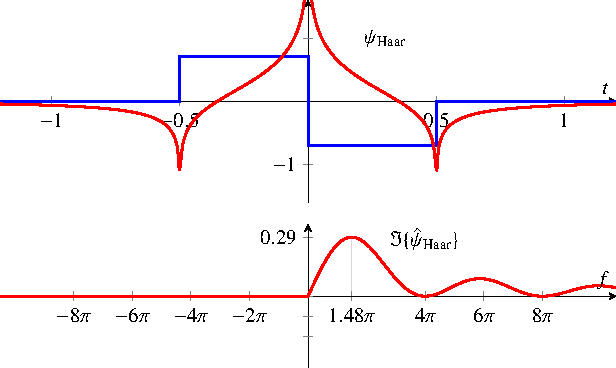
\includegraphics{papers/complex/images/ahaar.pdf}
	\caption{Das analytische Haar-Wavelet im Zeit- und Frequenzbereich.}
	\label{complex:ahaar}
\end{figure}

\begin{figure}
	\centering
	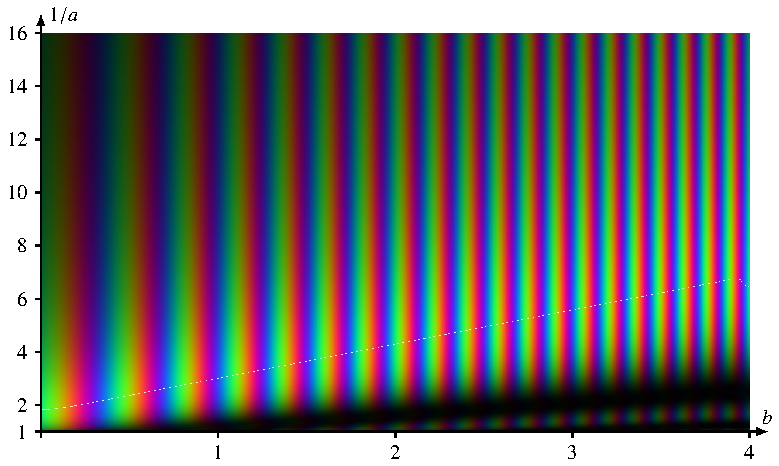
\includegraphics{papers/complex/images/chirp_ahaar.pdf}
	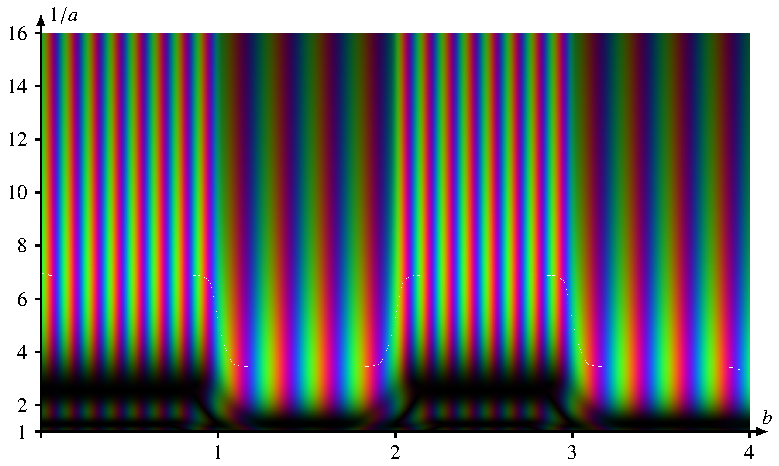
\includegraphics{papers/complex/images/square_ahaar.pdf}
	\caption{Farb-codierte Wavelet-Transformationen der beiden Beispielsignale mit dem \\ analytischen Haar-Wavelet.}
	\label{complex:ahaar-ex}
\end{figure}


\section{Zyklische Faltung, Signal-Padding und Performanz}
\rhead{Zyklische Faltung}
\label{complex:circ-conv-padding}
%% Effekt der zyklischen Faltung
%% Lösen durch padden des Signals
%%  - zero padding
%%  - padden durch spiegeln des Signals
%% Performanz-Vergleich anhand Matlab-Skript

\section{Schlussfolgerung}
\rhead{Schlussfolgerung}
%% Jedes Wavelet kann in ein analytisches transformiert werden
%% Die Wavelets aus der FWT sind allerdings für die CWT ungeeignet, 
%% da sie nich in geschlossener Form im Frequenzbereich berechnet werden können
%% (Aufstellen der Faltungs-Matrix)
%% Allerdings ist das Morlet-WAvelet auch zu bevorzugen, da es die optimale 
%% Schärfe zwischen Frequenz- und Zeitauflösung beitet (Gaus\ldots)

\printbibliography[heading=subbibliography]
\end{refsection}
